\documentclass[../main.tex]{subfiles}

% ======================== Document: Results ======================== %

\begin{document}
\section{Results}
\label{sec:results}

\subsection{Patent applications}

Table \ref{tab:dd_twfe_patents} presents results of the estimation of Equation \ref{eq:dd_model} using patent applications as the explained variable. Specification (1) includes a baseline result with no control variables. Specification (2) includes economic controls to account for factors that may affect the comparability of the treatment and control groups regarding firm activity and overall economic trends which vary across time and provinces. The number of foreign parties involved in patent applications is also included, to control for foreign influences. Specification (3) considers additional controls, which are included in case the previous ones did not account for differences in trends due to reasons other than the economy, or that economic activity is not well captured by standard economic variables in Specification (2). 

The DD estimate is the coefficient on Treatment \texttimes Post, showing that the intervention led to an -9.3\% to +1.1\% change in Alberta patent applications. The baseline and additional controls specifications show a negative effect, while the other specification shows a positive one. Only the baseline DD specification shows a statistically significant effect, which disappears after controlling for other factors. Standard errors for the coefficient of interest are small compared to those of the controls, showing that $\hat{\beta}$ is estimated with a fairly good level of precision. 
\begin{table}[htbp!]
    \centering
    \begin{threeparttable}
        \caption{Difference-in-differences (DD) specifications for quarterly patent applications}
        \label{tab:dd_twfe_patents}
        
\begin{tabular}[t]{lccc}
\toprule
  & (1) & (2) & (3)\\
\midrule
Treatment x Post & \num{-0.093}* & \num{0.001} & \num{-0.011}\\
\textbf{} & \textbf{(\num{0.042})} & \textbf{(\num{0.066})} & \textbf{(\num{0.076})}\\
Ln Full-time employment &  & \num{0.756} & \num{1.032}\\
 &  & (\num{0.644}) & (\num{0.646})\\
Ln Median wage &  & \num{1.235}** & \num{1.107}**\\
 &  & (\num{0.387}) & (\num{0.445})\\
CPI &  & \num{-0.015}** & \num{-0.007}\\
 &  & (\num{0.005}) & (\num{0.008})\\
Ln +1 Business insolvencies &  & \num{-0.065}** & \num{-0.051}*\\
 &  & (\num{0.027}) & (\num{0.023})\\
Ln Intl. exports &  & \num{-0.081} & \num{-0.079}\\
 &  & (\num{0.097}) & (\num{0.125})\\
Ln Intl. imports &  & \num{0.016} & \num{0.022}\\
 &  & (\num{0.126}) & (\num{0.127})\\
Ln Retail sales &  & \num{-0.279} & \num{0.094}\\
 &  & (\num{0.421}) & (\num{0.492})\\
Ln Wholesale sales &  & \num{-0.150} & \num{-0.229}\\
 &  & (\num{0.156}) & (\num{0.139})\\
Ln Manufacturing sales &  & \num{0.275} & \num{0.210}\\
 &  & (\num{0.153}) & (\num{0.146})\\
Ln +1 Foreign patent parties &  & \num{0.141}*** & \num{0.135}***\\
 &  & (\num{0.016}) & (\num{0.016})\\
Ln International travellers &  &  & \num{-0.129}***\\
 &  &  & (\num{0.034})\\
Ln Arriving vehicles &  &  & \num{0.007}\\
 &  &  & (\num{0.004})\\
Ln Electric power generation &  &  & \num{0.078}\\
 &  &  & (\num{0.115})\\
Ln Average actual hours &  &  & \num{0.109}\\
 &  &  & (\num{0.277})\\
New housing price index &  &  & \num{-0.003}\\
 &  &  & (\num{0.002})\\
Ln Food services receipts &  &  & \num{-0.080}\\
 &  &  & (\num{0.201})\\
Ln Average job tenure &  &  & \num{-0.424}\\
 &  &  & (\num{0.373})\\
\midrule
Explained variable &  & $\ln(\text{Patents}+1)$ & \\
$N$ & \num{656} & \num{656} & \num{656}\\
Adj. $R^2$ & \num{0.975} & \num{0.980} & \num{0.980}\\
Adj. within $R^2$ & \num{0.002} & \num{0.205} & \num{0.210}\\
RMSE & \num{0.206} & \num{0.182} & \num{0.180}\\
\bottomrule
\end{tabular}
}
        \begin{tablenotes}
            \small
            \item \textit{Notes}: Clustered standard errors at the province and quarter level shown in parentheses. All specifications include fixed effects for provinces and quarters. ***$p<0.01$, **$p<0.05$, *$p<0.1$.
        \end{tablenotes}
    \end{threeparttable}
\end{table}

I display the results of the event study regressions in Figure \ref{fig:event_study_patents}, which plots the $\hat{\beta}_t$ interaction coefficients in \ref{eq:event_study} with the same controls as the specifications in Table \ref{tab:dd_twfe_patents}. For specifications (2) and (3) there is no significant difference in patent applications between treatment and control groups for most pre-intervention periods. This supports the key identifying assumption of the DD design, supporting the causal identification of $\hat{\beta}$. The baseline model does show several pre-policy periods where the treatment and control groups diverge, underscoring the importance of including controls in the model. However, in all specifications, there are particular periods for which a statistically significant difference exists. This can be due to random noise or to a temporary real effect. Since it is only one period that disappears later, I do not consider it as a substantial threat to the causal identification of $\hat{\beta}$. 
Regarding the effect of the policy itself, results point toward an overall null effect in the event study plots as well. There are marginally negative effects on some periods, which appear next to periods with null effects. This evidence supports the null effect found in the DD specifications (2) and (3), which is consistent with the fact that economic factors (such as business insolvencies, wage, employment, etc.) and foreign influences (the number of foreign parties in patent applications) control for differences between treated and untreated observations.

\begin{figure}[htbp!]
    \centering
    \caption{Event study plots for quarterly patent applications}
    \label{fig:event_study_patents}
   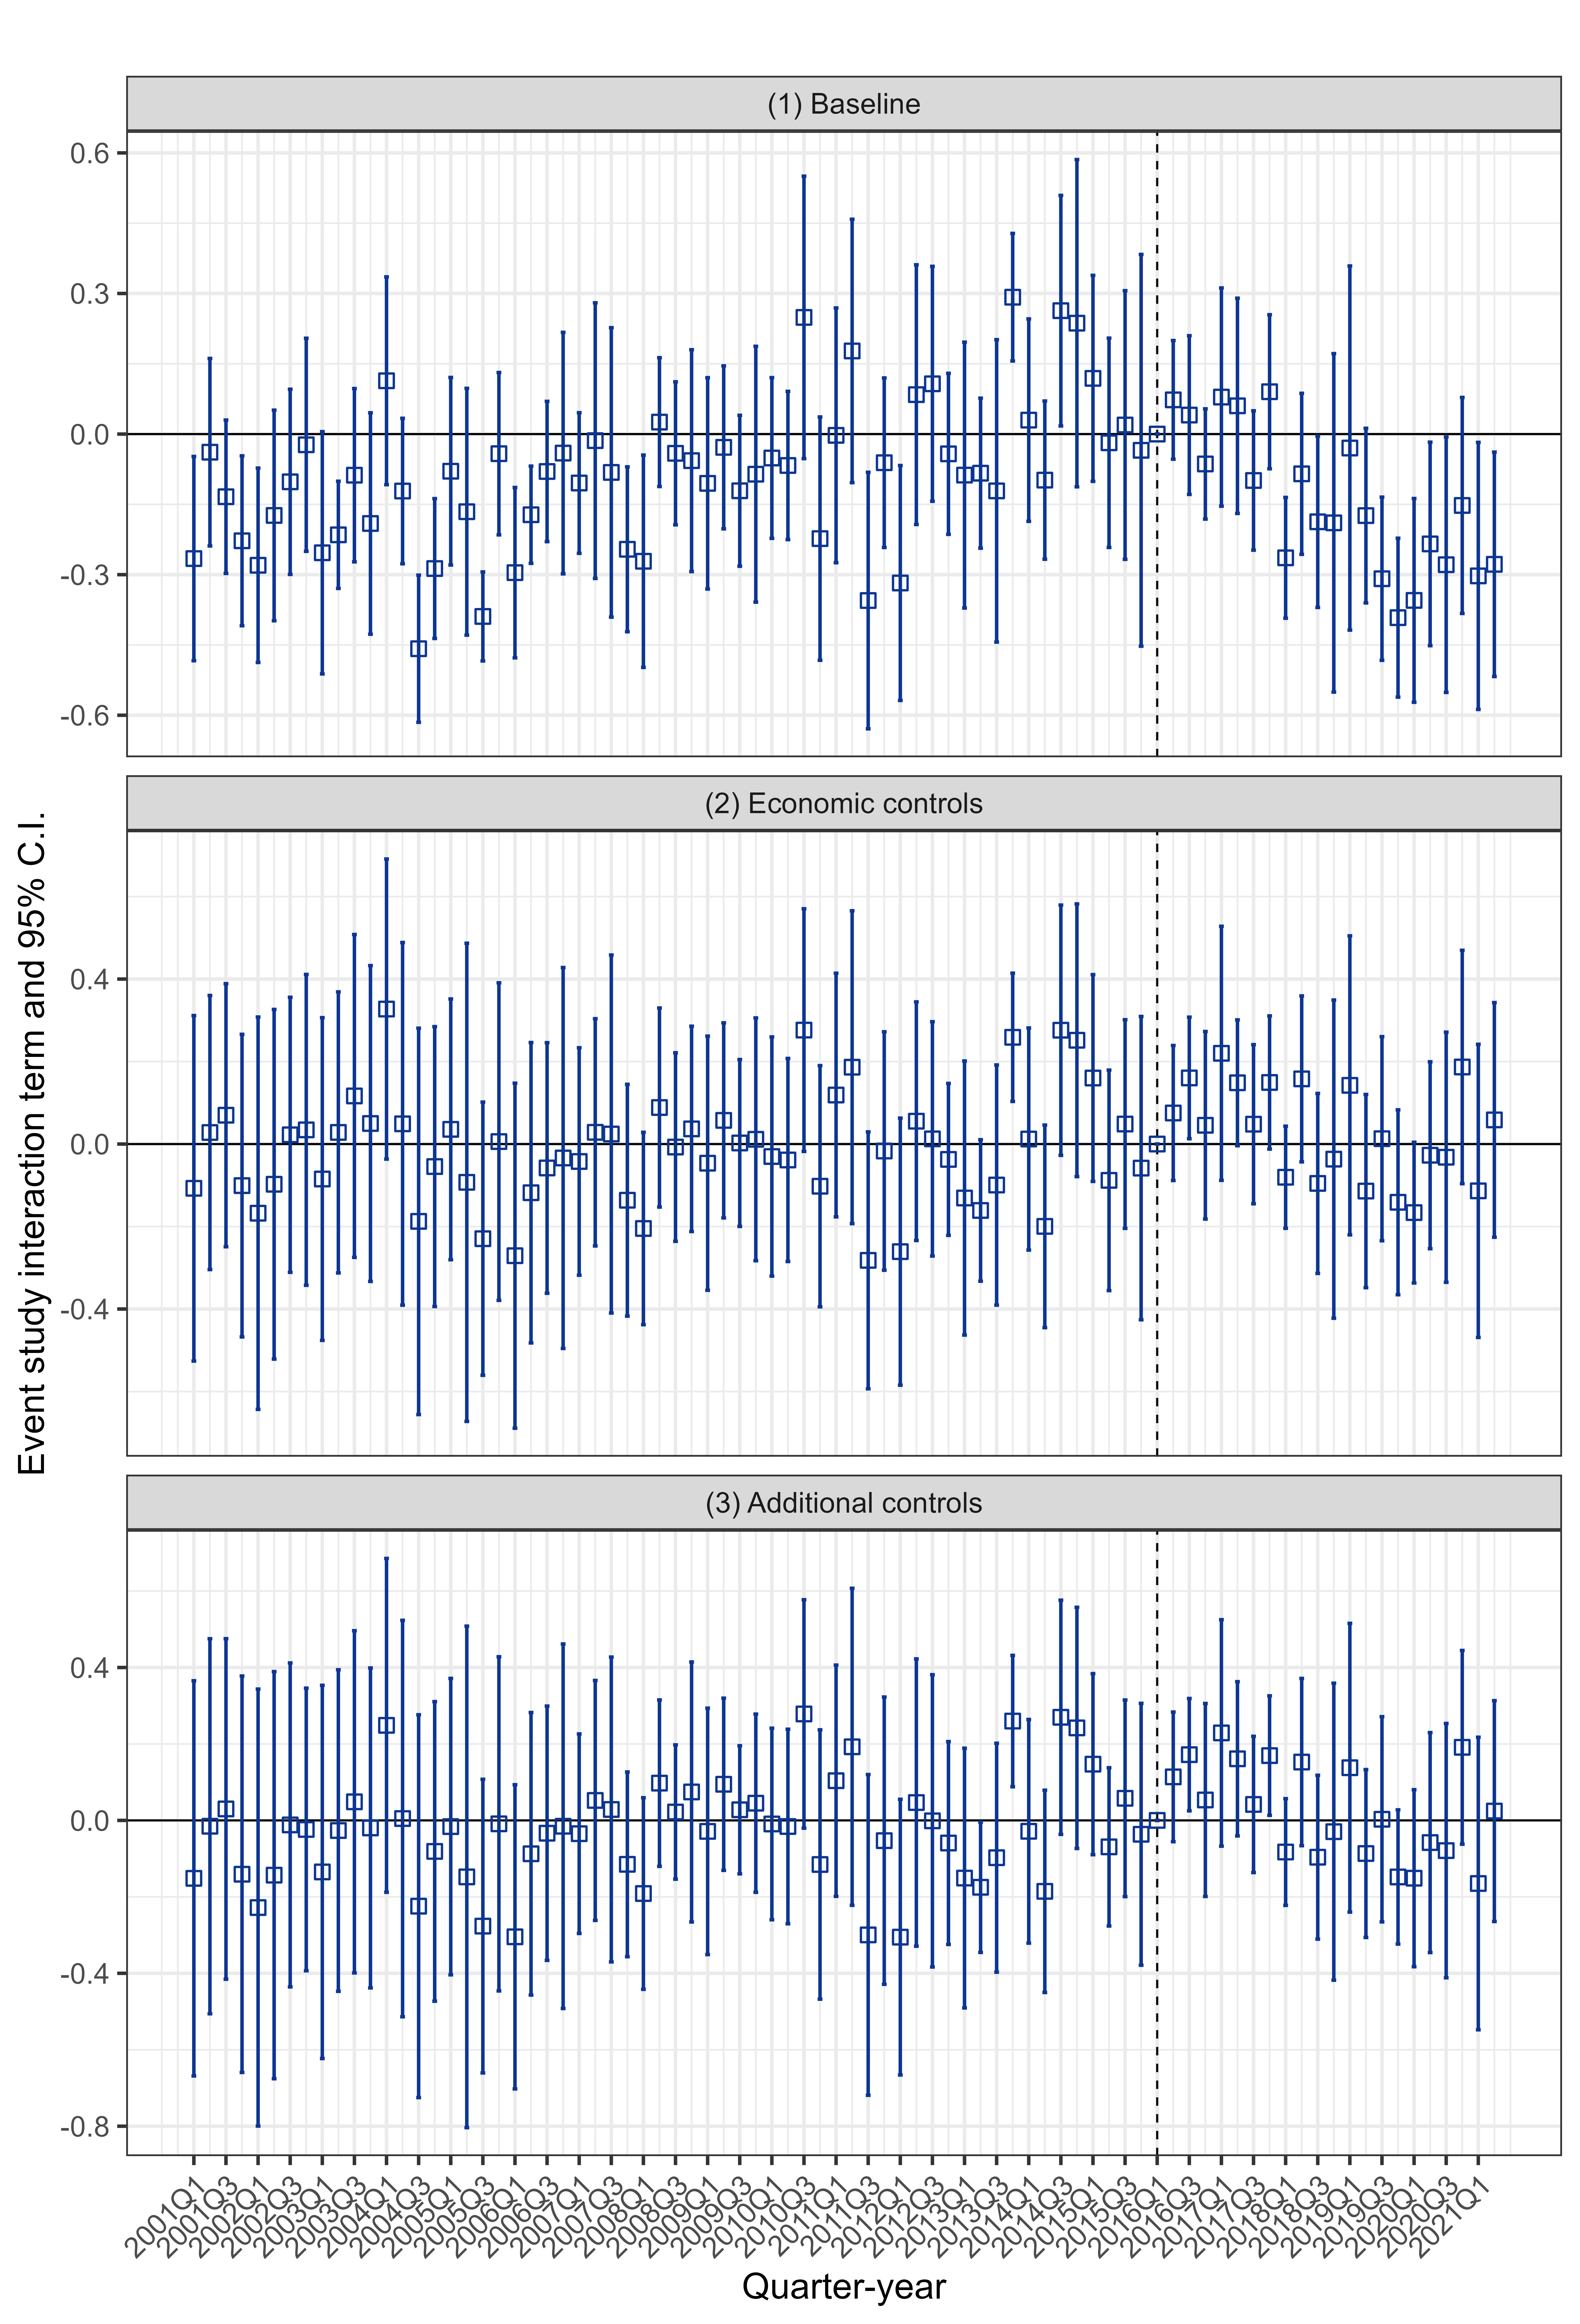
\includegraphics{\subfix{../../figures/event-studies/quarterly/patents_faceted.png}}
    \begin{minipage}{0.9\textwidth}
        \footnotesize
        \textit{Notes}: The figure shows the estimated coefficients of the interaction term between period and treatment binary variables in Equation \ref{eq:event_study} for each quarter. The points represent the point estimate, while the error bars represent the 95\% confidence cluster-robust interval. The vertical line represents the start of the AITC intervention in 2017Q1, with the reference level being the quarter before the intervention. Baseline, economic, and additional controls specifications include the controls seen in specifications (1) through (3) in Table \ref{tab:dd_twfe_patents}. 
    \end{minipage}
\end{figure}

\subsection{Separating by International Patent Classifications (IPC)}

\begin{table}[htbp!]
    \centering
\begin{threeparttable}
    \caption{Difference-in-differences results for quarterly patent applications by IPC section}
    
\begin{tabular}[t]{lcccccccc}
\toprule
  & (1) & (2) & (3) & (4) & (5) & (6) & (7) & (8)\\
\midrule
Treatment x Post & \num{0.427}*** & \num{0.366} & \num{0.066} & \num{0.235} & \num{-0.530}*** & \num{0.167} & \num{-0.083} & \num{0.209}\\
\textbf{} & \textbf{(\num{0.071})} & \textbf{(\num{0.195})} & \textbf{(\num{0.171})} & \textbf{(\num{0.132})} & \textbf{(\num{0.045})} & \textbf{(\num{0.106})} & \textbf{(\num{0.187})} & \textbf{(\num{0.135})}\\
\midrule
Patent section (IPC) & A & B & C & D & E & F & G & H\\
$N$ & \num{656} & \num{656} & \num{656} & \num{656} & \num{656} & \num{656} & \num{656} & \num{656}\\
Adj. $R^2$ & \num{0.913} & \num{0.911} & \num{0.879} & \num{0.353} & \num{0.914} & \num{0.875} & \num{0.910} & \num{0.908}\\
Adj. within $R^2$ & \num{0.111} & \num{0.056} & \num{0.082} & \num{0.033} & \num{0.061} & \num{0.021} & \num{0.060} & \num{0.063}\\
RMSE & \num{0.324} & \num{0.355} & \num{0.381} & \num{0.356} & \num{0.361} & \num{0.394} & \num{0.395} & \num{0.409}\\
\bottomrule
\end{tabular}
}
    \label{tab:dd_twfe_patents_by_section}
    \begin{tablenotes}
        \footnotesize
        \item \textit{Notes:} All specifications include controls in Specification (3) of Table \ref{tab:dd_twfe_patents}, not shown for brevity, and fixed effects for provinces and quarters. Clustered standard errors at the province and quarter level shown in parentheses. 
        \item Sections of the IPC are A: Human Necessities, B: Performing Operations; Transporting, C: Chemistry; Metallurgy, D: Textiles; Paper, E: Fixed Constructions, F: Mechanical Engineering; G: Physics, H: Electricity. Patents with multiple sections are not included. ***$p<0.01$, **$p<0.05$, *$p<0.1$.
    \end{tablenotes}
\end{threeparttable}
\end{table}

In Table \ref{tab:dd_twfe_patents_by_section}, I present the results of estimating Equation \ref{eq:dd_model} allowing for heterogeneity by IPC section and including the controls of Specification (3) in Table \ref{tab:dd_twfe_patents}. The results show that the AITC intervention had a null effect on most of the IPC sections except A, D and E, corresponding to human necessities, textile/paper and fixed construction inventions. The effect on section A and D inventions is positive while on section E it is negative. 

Approximately, it would appear that the positive effect on human necessity and textile applications is larger than the negative effect on fixed construction applications. However, given that there is a smaller number of patents per IPC section for all provinces in every period, I am underpowered to detect small effects on other sections, which could also be negative, thus explaining the null effect on total patents. The event study regressions in Figure \ref{fig:event_study_patents_section} provide additional insight about the intervention's effect on patent applications by IPC section. The figure displays the same coefficients and confidence intervals as those of in Figure \ref{fig:event_study_patents} now separating by IPC section and restricting to the additional controls specification. 

Human necessity (A) inventions, which include agriculture, medicine and apparel-related inventions, saw a greater amount of patent applications in most post-intervention periods compared to the control group. However, pre-intervention periods do not provide evidence in support of the common trends assumption, which may be driving a spurious positive effect in the post-intervention periods. Regarding textile and paper (D) inventions, the event study plot shows very large increases in patent applications in some intervention periods compared to the control group. However, these increases are confined to the last few periods, with the first quarters after the intervention showing no significant differences.

The offsetting negative effect on fixed construction (E) inventions is difficult to interpret in the event study plot. Almost no post-intervention period shows a significant difference between the treatment and control groups. However, the DD specification picks up a negative effect because of large positive differences in the pre-intervention periods. I cannot reject that the negative effect is due to factors other than the AITC intervention. 

In general, while the DD estimates would point to a significant effect of the AITC on some IPC section patent applications, closer inspection of the event study plots shows that the effect cannot be supported by a common trends assumption. Other factors may be driving the results which are unobserved in the data and specific to these inventions.
   
\begin{figure}[htbp!]
    \centering
    \caption{Event study plot for quarterly patent applications by IPC section}
    \label{fig:event_study_patents_section}
    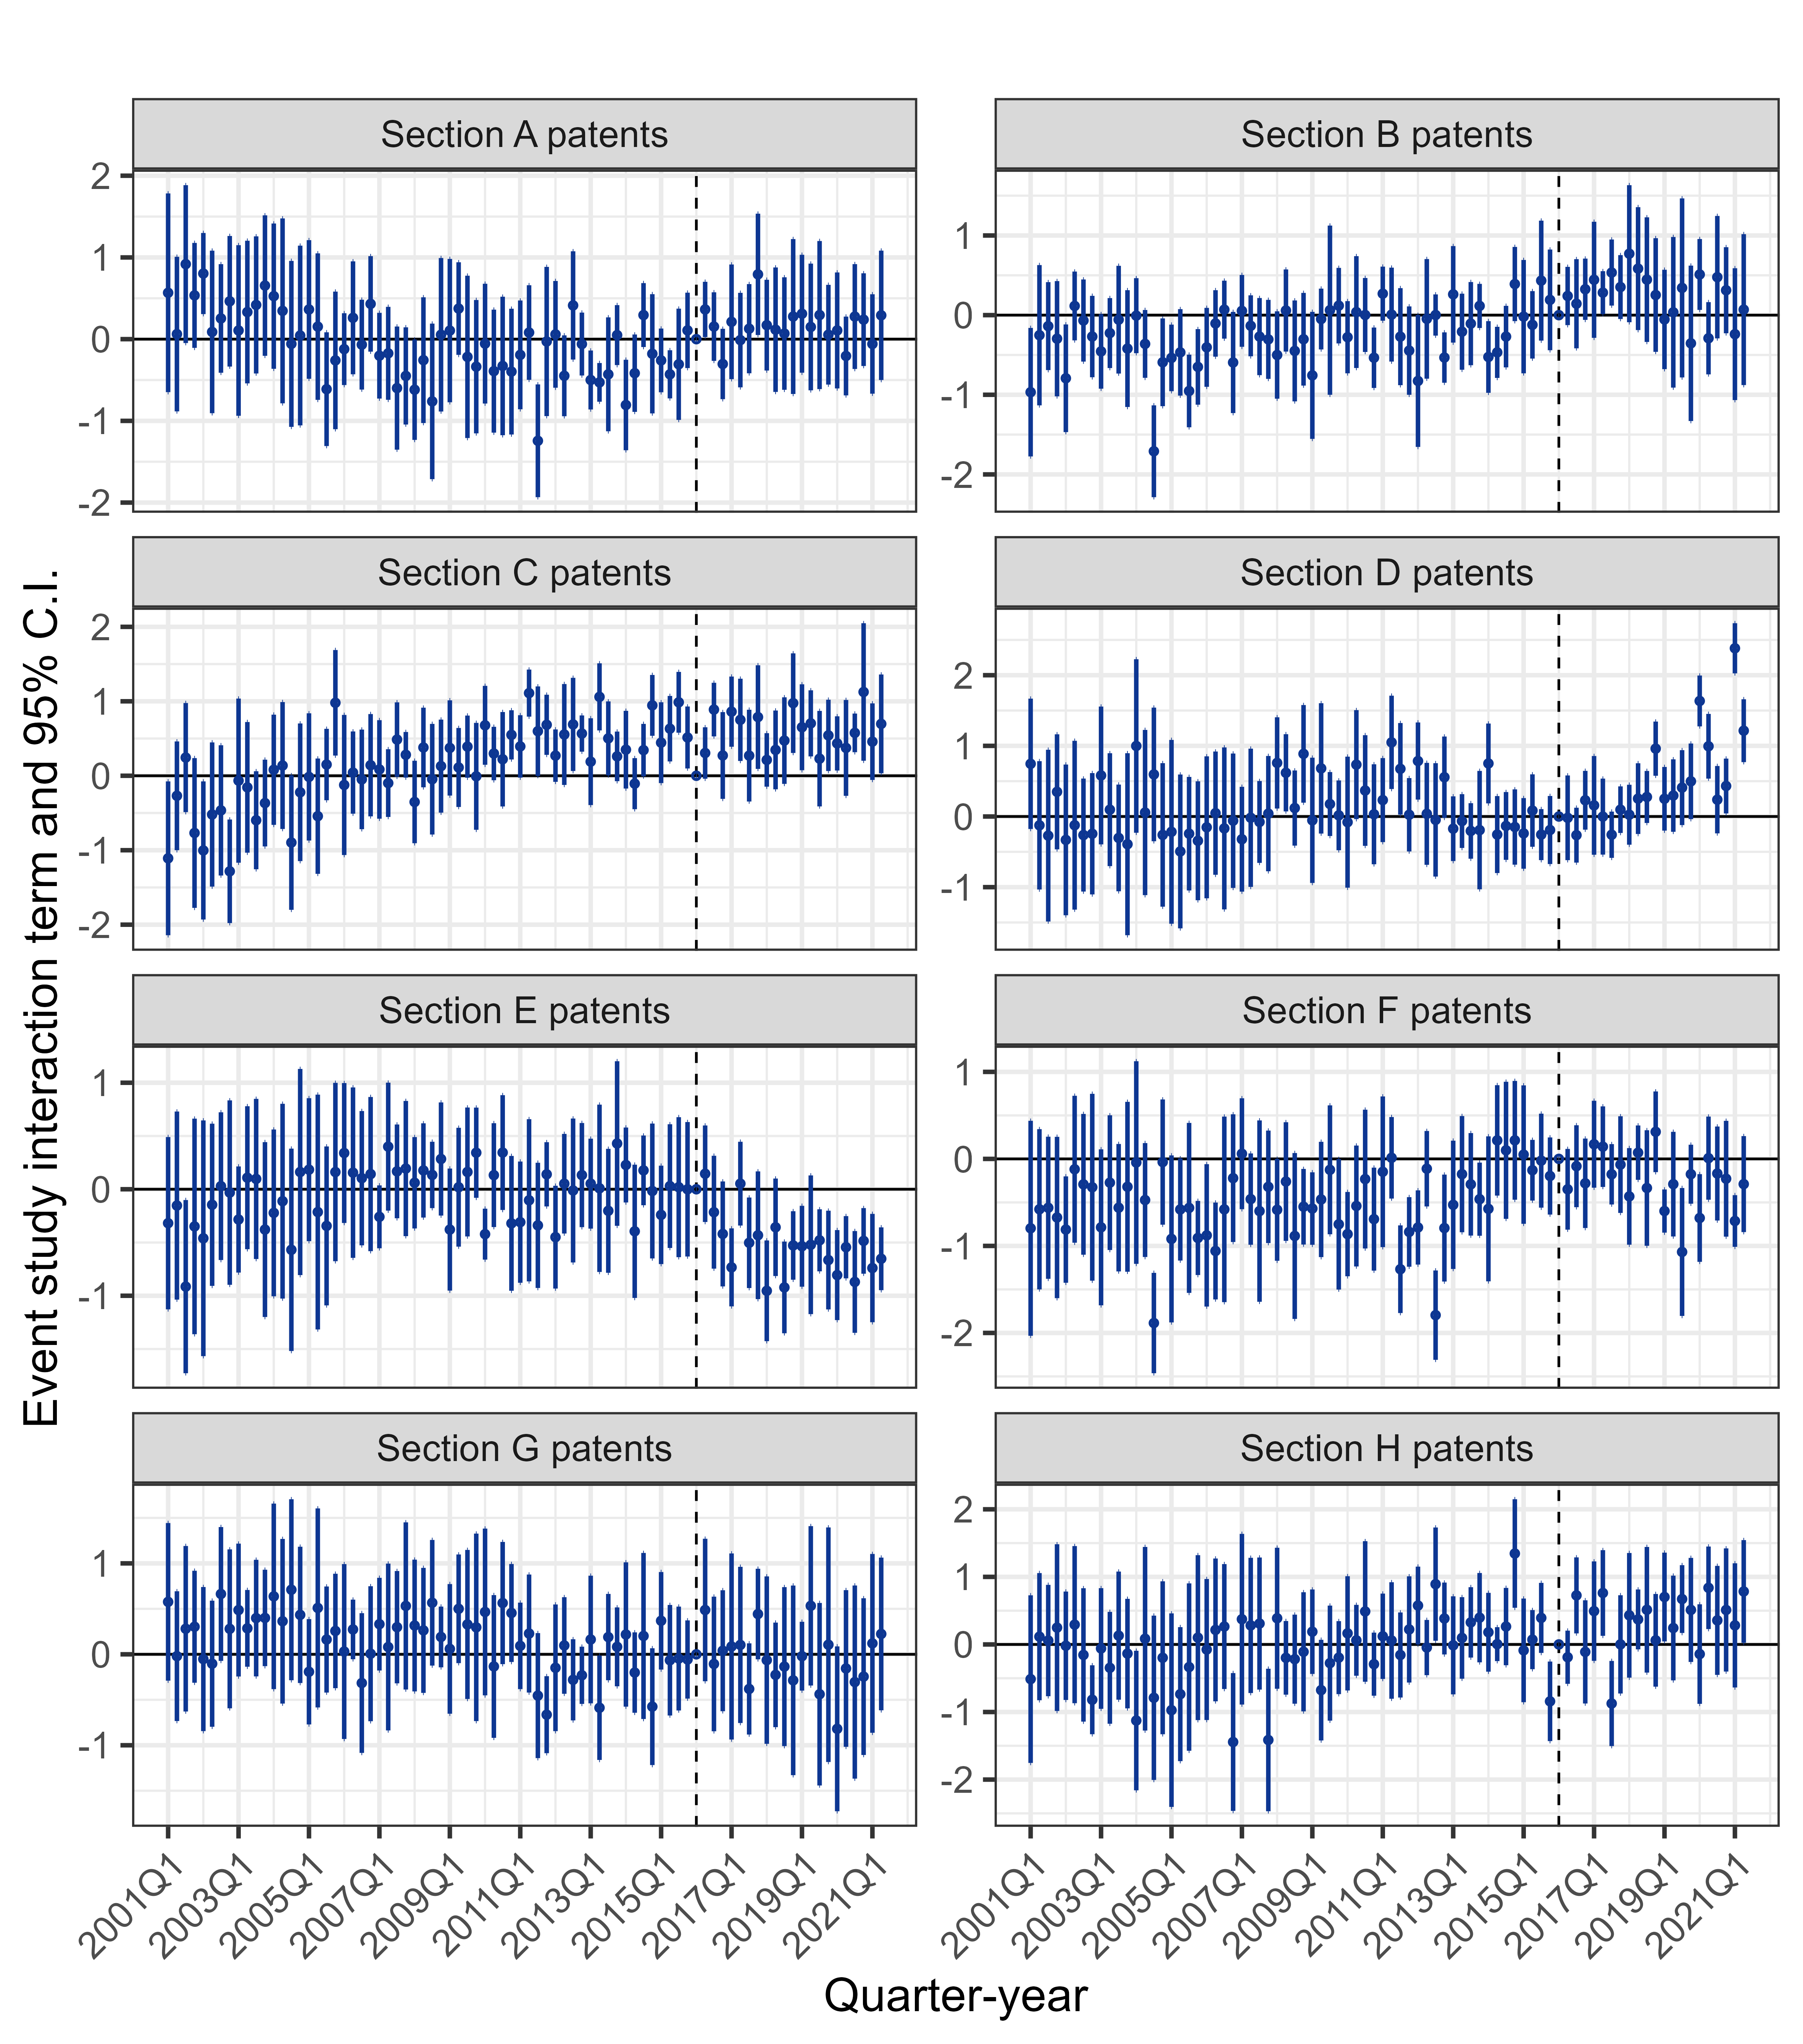
\includegraphics{\subfix{../../figures/event-studies/quarterly/patent_sections_faceted.png}}
    \begin{minipage}{0.9\textwidth}
        \footnotesize
        \textit{Notes}: The figure shows the estimated coefficients of the interaction term between period and treatment binary variables in Equation \ref{eq:event_study} for each quarter, separating by IPC section. The points represent the point estimate, while the error bars represent the 95\% confidence cluster-robust interval. The vertical line represents the start of the AITC intervention in 2017Q1 with the reference level being the quarter before the intervention. Controls are the same as those in Specification (3) in Table \ref{tab:dd_twfe_patents}. 
    \end{minipage}
\end{figure}

\subsection{Robustness checks}

Appendix \ref{sec:appendixb} presents the results of the DD specifications and event studies for number of parties in patent applications as explained variables. All models use the controls in Specification (3) of Table \ref{tab:dd_twfe_patents}. I consider total parties in patent applications and also separate by specific types: inventors, owners and applicants. All DD specifications show a null effect of the policy with a slight increase in standard errors. This is understandable given that the number of interested parties as an explained variable proxies for both the number of patent applications in a province but also for the size of the application team. This makes the use of the natural logarithm transformation crucial for a better interpretation of the DD estimate, as the the number of parties is an inflated indicator of innovation. 

Event study plots show that the effect is null for all post-policy periods for total parties, applicants and owners. Pre-policy trends show less consistency between treatment and control groups compared to patent applications, particularly in 52 to 36 periods before the AITC started. Because this difference disappears in the following quarters, I do not see it as a substantial threat to causal identification. Overall, patent application counts behave similarly to parties within patent applications in both the DD and event study regressions. This means that my mapping of patents to provinces does not drive my results.

Appendix \ref{sec:appendixc} reproduces the DD specifications and event study regression using the province-month panel. Monthly DD specifications show a null effect of the AITC intervention on the log of patent applications, considering all three specifications in Table \ref{tab:dd_twfe_patents} (baseline, economic and additional controls). The same is true for IPC sections. This means that the additional precision does not change the existence of a null result. 

Regarding the event study plot, the pre-intervention months are much less stable than in the quarterly case. There are statistically significant differences in many periods before January 2017, which present themselves in an almost seasonal nature: differences start being relatively large, but as months pass they become smaller until being null. This explains why the quarterly aggregation does not show an unstable pre-intervention trend. I discuss the implications of this issue in the conclusion. In the post-intervention periods, there were months in which Alberta had less patent applications than the control provinces, but in the last period, these differences were not significant. Overall, post-intervention periods do not show a significant deviation from the quarterly results.

\end{document}